%%%%%%%%%%%%%%%%%%%%%%%%%%%%%%%%%%%%%%%%%
% Structured General Purpose Assignment
% LaTeX Template
%
% This template has been downloaded from:
% http://www.latextemplates.com
%
% Original author:
% Ted Pavlic (http://www.tedpavlic.com)
%
% Note:
% The \lipsum[#] commands throughout this template generate dummy text
% to fill the template out. These commands should all be removed when 
% writing assignment content.
%
%%%%%%%%%%%%%%%%%%%%%%%%%%%%%%%%%%%%%%%%%

\documentclass{article}

\usepackage{fancyhdr} % Required for custom headers
\usepackage{lastpage} % Required to determine the last page for the footer
\usepackage{extramarks} % Required for headers and footers
\usepackage{graphicx} % Required to insert images
\usepackage[utf8]{inputenc}

% Margins
\topmargin=-0.45in
\evensidemargin=0in
\oddsidemargin=0in
\textwidth=6.5in
\textheight=9.0in
\headsep=0.25in 

\linespread{1.1} % Line spacing



\setlength\parindent{0pt} % Removes all indentation from paragraphs

%----------------------------------------------------------------------------------------
%	DOCUMENT STRUCTURE COMMANDS
%	Skip this unless you know what you're doing
%----------------------------------------------------------------------------------------

% Header and footer for when a page split occurs within a problem environment
\newcommand{\enterProblemHeader}[1]{
\nobreak\extramarks{#1}{#1 continued on next page\ldots}\nobreak
\nobreak\extramarks{#1 (continued)}{#1 continued on next page\ldots}\nobreak
}

% Header and footer for when a page split occurs between problem environments
\newcommand{\exitProblemHeader}[1]{
\nobreak\extramarks{#1 (continued)}{#1 continued on next page\ldots}\nobreak
\nobreak\extramarks{#1}{}\nobreak
}

\setcounter{secnumdepth}{0} % Removes default section numbers
\newcounter{homeworkProblemCounter} % Creates a counter to keep track of the number of problems

%----------------------------------------------------------------------------------------
%	NAME AND CLASS SECTION
%----------------------------------------------------------------------------------------

\newcommand{\lessonNumber}[1]{Lezione\ \##1} % Assignment title
\newcommand{\lessonDate}[4]{#1,\ #2\ #3\ #4} % Due date
\newcommand{\lessonCourse}[1]{#1} % Course/class
\newcommand{\lessonTime}[1]{#1} % Class/lecture time
\newcommand{\lessonTeacher}[1]{#1} % Teacher/lecturer
\newcommand{\lessonAuthor}[1]{#1} % Your name
\begin{document}

\section{Qualità di processo(7)}
\textit{Controllo} = \textbf{Governance:} gestione strategica.

Dobbiamo crearci regole per il miglioramento dei processi, migliorandoli in:
\begin{itemize}
	\item \textbf{Efficacia:} prodotti conformi alle attese;
	\item \textbf{Efficienza:} minori costi a pari qualità di prodotto; 
\end{itemize} 

\textbf{Norme ISO 9000-1:} suggeriscono un sistema di valutazione di qualità.\\
\textbf{Piano di Qualifica:} documento che definisce gli elementi del Sistema Gestione Qualità (SGQ) e le risorse che devono essere applicate in uno specifico caso (prodotto, processo, progetto).

Ci sono vari tipi di strumenti di valutazione:
\begin{itemize}
	\item \textbf{SPY:} si attua una valutazione oggettiva dei processi di un'organizzazione per darne un giudizio di maturità e individuare azioni migliorative. Educa la strategia a tentativi;
 	\item \textbf{CMMI:}
 		\begin{itemize}
 			\item \textbf{CAPABILITY:} misura quanto è adeguato un processo per gli scopi per cui è stato definito, l'intorno del risultato di efficienza ed efficacia raggiungibile utilizzando quel processo;
 			\item \textbf{MATURITY:} misura di quanto è governato il sistema dei processi dell'azienda. Risulta dell'effetto combinato delle capability dei processi coinvolti;
 			\item \textbf{MODEL:} insieme di requisiti via via più stringenti per valutare il percorso di miglioramento dei processi dell'azienda;
 			\item \textbf{INTEGRATION:} architettura di integrazione delle diverse discipline e tipologie di attività delle aziende.
 		\end{itemize}
 		educa la strategia a priori.
	
\end{itemize} 
Si dice che un'organizzazione capace di effettuare miglioramenti sui processi è in grado di fare \textbf{governance}, sinonimo di efficacia, efficienza, mantenibilità e visione. Gestire la qualità di processi non sta al Project Manager ma ad uno strato più importante che sta sopra e ha una visione più ampia e possiede una strategia di lungo periodo riferita al miglioramento.

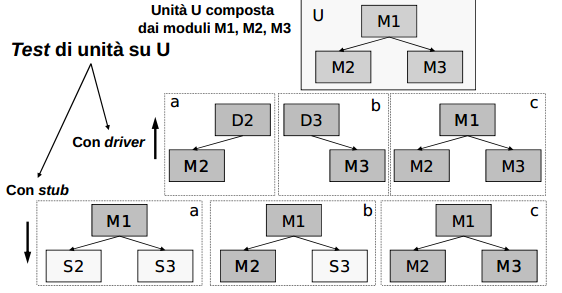
\includegraphics[width=0.75\columnwidth]{img3.png} % Example image

\begin{enumerate}
	\item Si parte da osservare che al piano terra c'è uno strato iniziale in cui tutti all'inizio si collocano. I processi, se ci sono, sono a questo stadio \textbf{unpredictable}, impredicibili, \textbf{poorly controlled} e \textbf{reacted}.
	\item Il livello 2 è \textbf{managed}, cioè gestito. I processi esistono nei progetti e rimangono prevalentemente reattivi.
	\item  Il livello 3 è \textbf{definito}, i processi sono proattivi, esistono trasversalmente, manca ancora il miglioramento.
	\item Il livello 4 introduce misurazione rispetto al controllo e si chiama \textbf{quantitatively managed}.
	\item Al livello 5 non soltanto misuriamo ma miglioriamo, \textbf{optimizing}.
\end{enumerate}
\end{document}